% The "%" character denotes a comment
% This file was written by Nathan Moore, Winona State University
% as a template for how lab reports might be written in LaTeX.
% style choices originally come from the American Journal of Physics's
% sample submission file, http://ajp.dickinson.edu/Contributors/manFormat.html
%
%
\documentclass[prb,preprint]{revtex4-1}
\usepackage{amsmath}  % needed for \tfrac, \bmatrix, etc.
\usepackage{amsfonts} % needed for bold Greek, Fraktur, and blackboard bold
\usepackage{graphicx} % needed for figures

%these are some macros (shortcuts)
\newcommand{\bea}{\begin{eqnarray}}
\newcommand{\eea}{\end{eqnarray}}
\newcommand{\be}{\begin{equation}}
\newcommand{\ee}{\end{equation}}

\begin{document}

\title{Electronics Lab 09: Common Emitter Amplifier and Infrared Detector}
\author{Adam Stammer}
%\email{adam.stammer@go.winona.edu}

\date{\today}

%if you include an abstract, it goes here
\begin{abstract}
Labs 9, 10, and 11 worked hand in hand to develop and test our understanding of Bipolar Junction Transistors in the active region. First, we took measurements with various resistors to see how beta changes with base current. From this data we were able to extrapolate a beta for a slightly different transistor circuit, also in the active region. Our estimation was reasonably close to the actual beta. Using this understanding we then designed a circuit using a phototransistor sensitive to infrared light such that the signals from a remote control might be decoded by a microcontroller. 
\end{abstract}

\maketitle


%These are my general reccomendations for an undergraduate lab report in Physics. 
%
%\textbf{Purpose}
%The lab report should start with a purpose statement.  Briefly 
%provide the necessary background and explain what problem your are trying to 
%solve/investigate.
%
%\textbf{Conclusions} Don't be coy, cut to the point right away and state what you found. This should be breif.
%
%\textbf{Theory} We never just measure stuff in Physics.  There's always a 
%theoretical idea behind the measurement we're making.  Explain  the ideas 
%behind your work, starting at the level of a successful Physics 221/222 
%student.
%
%\textbf{Data} Sketch out, in words and pictures, the apparatus you used to take data.  Report the data, graphically, if possible, and state the uncertainties  in your measurement.  Don't provide pages of computer printout here. Data tables shouldn't be your first choice when it comes to communicating your measurements.\cite{Tufte}
%
%\textbf{Analysis} With data presented, describe how the theory agrees/disagrees with 
%the data you took.  Normally this is accomplished with a fit line (or math 
%model) that is interpreted.
%
%\textbf{Limitations and Recommendations} Every measurement has limitations and it is only honest to report them to the reader.  ``Human Error'' is a meaningless statement.  After your analysis is complete, revisit the purpose statement.  This is the place to more forcefully argue your conclusions.    
%
%Notes: 
%Writing in the first person, eg ``I" or ``We," is fine.
%
%\newpage
%\textbf{Example Lab Report:}

\section{Collecting Data}
The circuit from which data was collected can be seen below, where $R_{B}$ is varied, $R_{C}=1k\Omega$, and $V_{cc}=15 Volts$. 

\begin{figure}[ht]
	\centering
	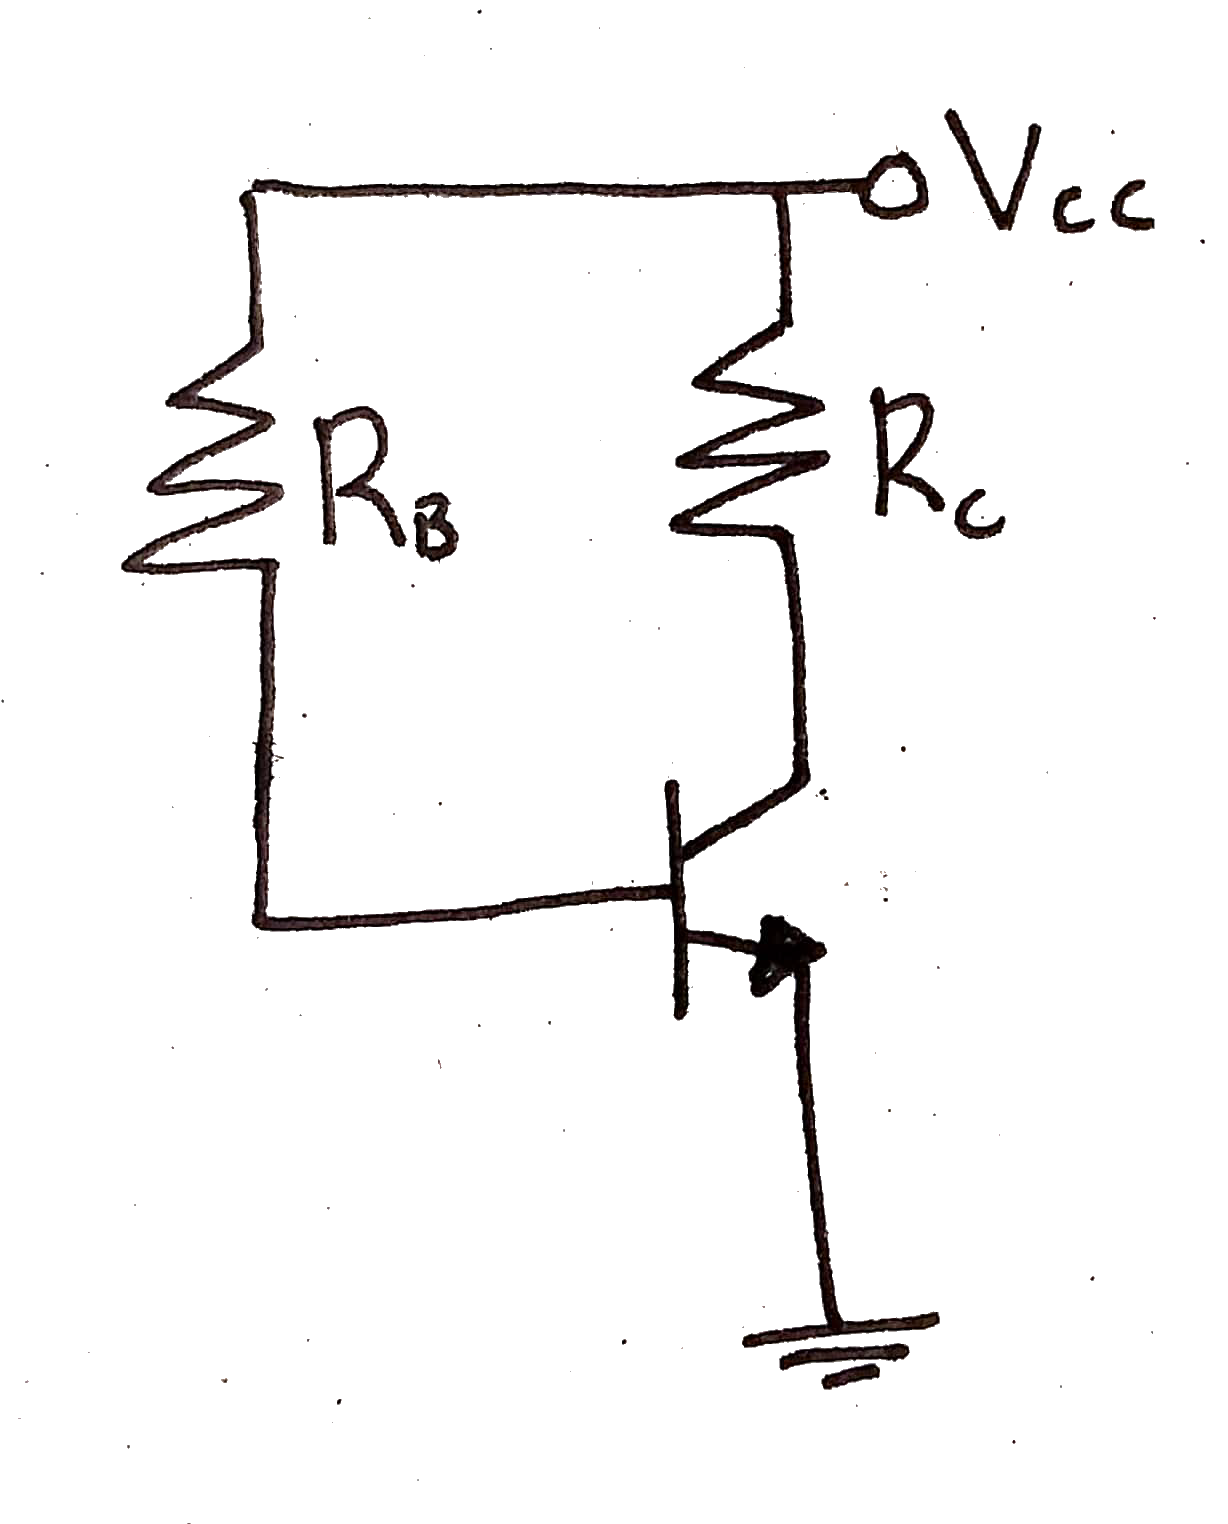
\includegraphics[width=2.5in]{c9.png}
	\caption{Circuit Used to Collect Data (Lab 9)}
	\label{fig1}
\end{figure}

Measuring $I_{B}$ and $I_{C}$ allows us to solve for $\beta$ since we know that $\beta=\frac{I_{C}}{I_{B}}$. Measuring $V_{CE}$ is also important as we don't know which if any of these resistor values put us in the active region, which is what we really care about here. The measurements collected can be seen below.

\begin{center}
\begin{tabular}{|c|c|c|c|c|}
	\hline
	\multicolumn{5}{|c|}{Circuit 1: Measurements}\\
	\hline
	$R_{B}(\Omega)$ & $I_{B}(mA)$ & $I_{C}(mA)$ & $\beta$ & $V_{CE}(V)$ \\
	\hline
	1.0M & .01 & 3.77 & 0 & 11.27 \\
	470k & .03 & 7.98 & 0 & 7.09 \\
	100k & .13 & 15 & 0 & .214 \\
	47k & .3 & 15.17 & 0 & .149 \\
	\hline
\end{tabular}
\end{center}

This data was then graphed. Since the first measurements when $R_{B}=47k\Omega$ seem to fall in the saturation region, I believe this data will negatively skew the extrapolation results, as we're only seeking a linear fit within the active region. Below you can see the graph of this data and the respective trendlines, the solid line with all of the data points, and the dashed line with the saturation region data point removed. From here it is assumed that the active only trendline will prove better at predicting beta, but lab 10 will test this theory.

\begin{figure}[ht]
	\centering
	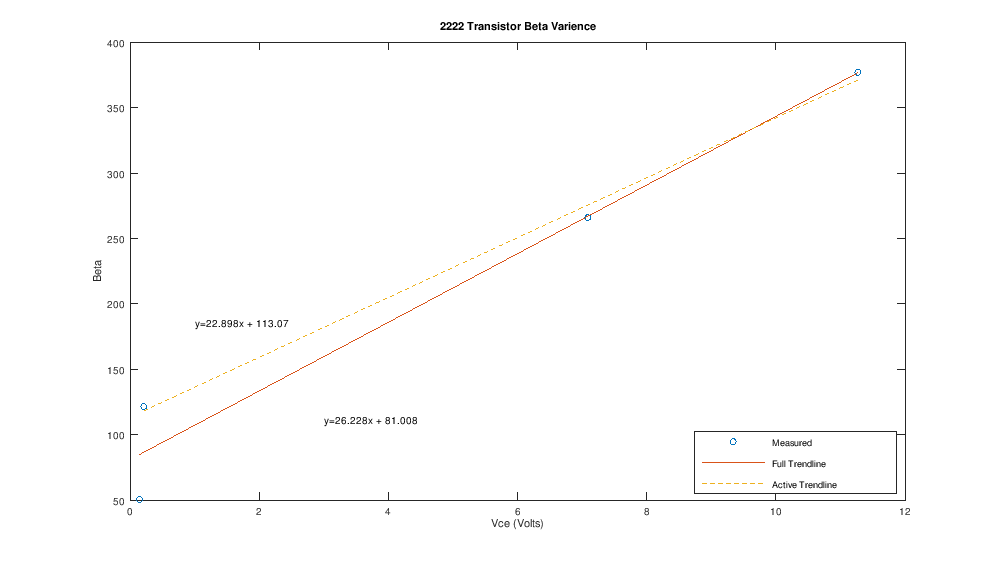
\includegraphics[width=6in]{9/bigGraph.png}
	\caption{Circuit Used to Collect Data (Lab 9)}
	\label{fig1}
\end{figure}

\section{Extrapolation Test}
Lab 10 uses a slightly different circuit, seen below, to test the fitlines we found above. $R_{1}=20k\Omega$, $R_{2}=10k\Omega$, $R_{C}=1k\Omega$, $R_{E}=1k\Omega$, $V_{cc}=15V$.


\begin{figure}[ht]
	\centering
	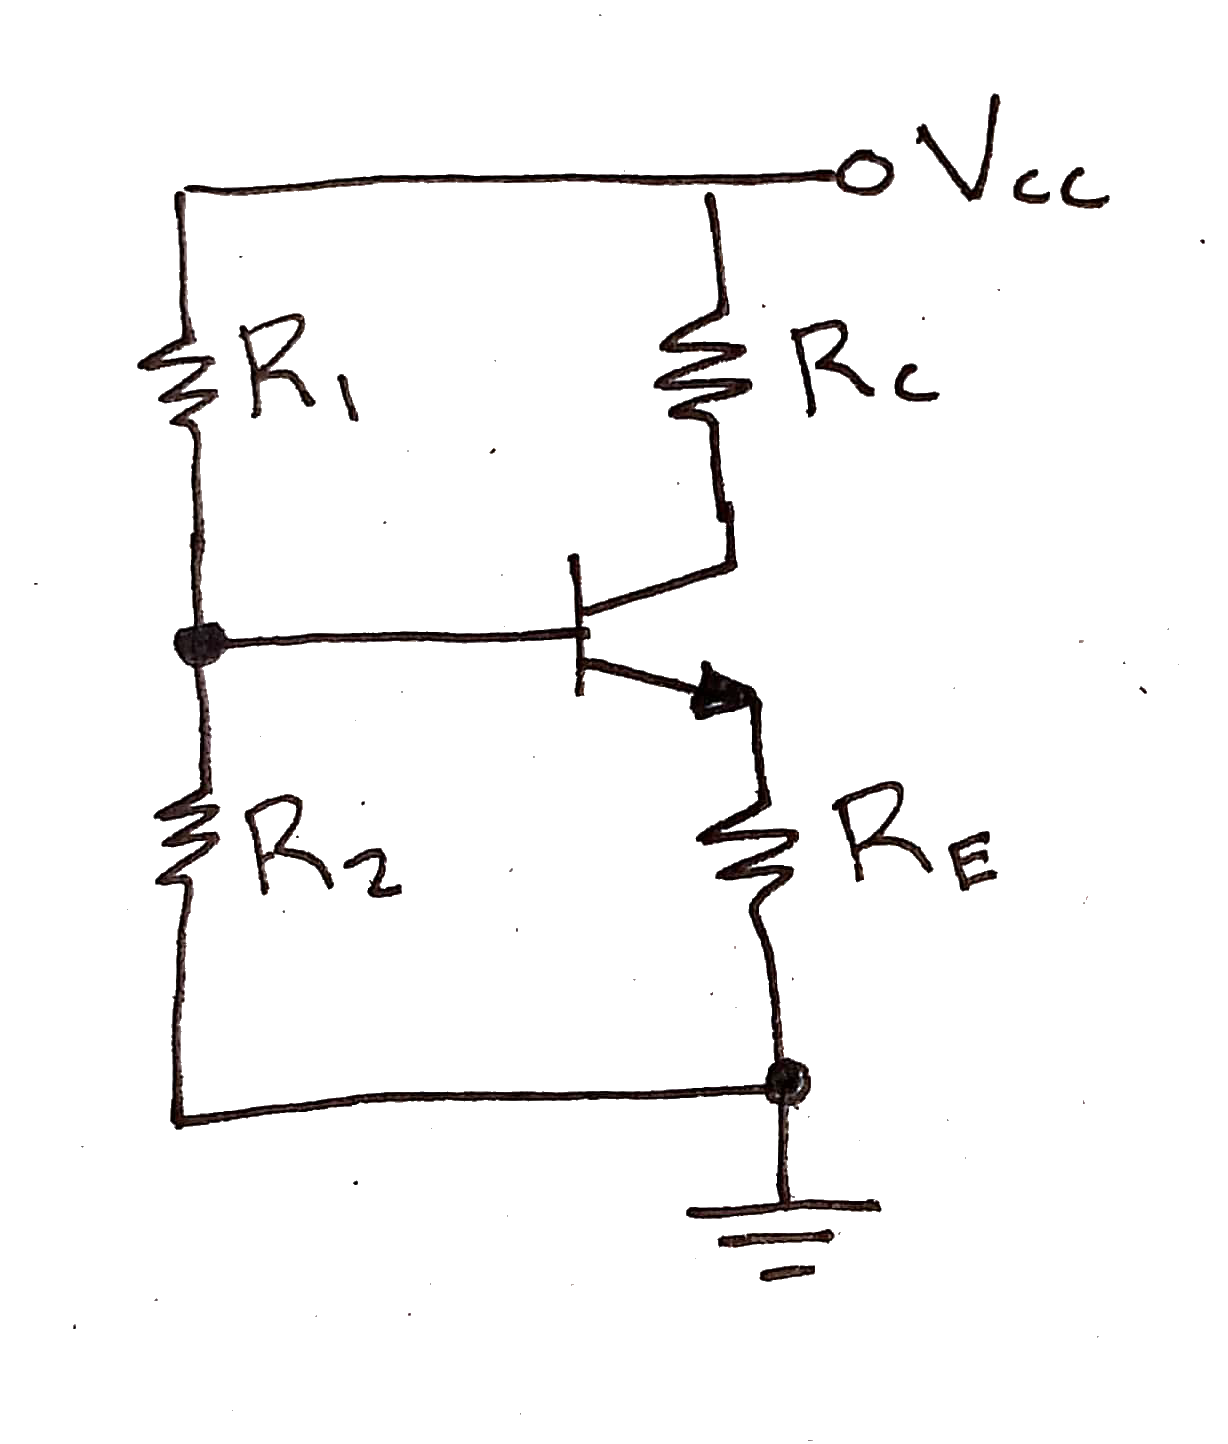
\includegraphics[width=2.5in]{c10.png}
	\caption{Circuit Used to Test Trendlines (Lab 10)}
	\label{fig1}
\end{figure}

From this circuit the following measurements were collected.

\begin{center}
	\begin{tabular}{|c|c|c|}
		\hline
		\multicolumn{3}{|c|}{Circuit 2: Measurements}\\
		\hline
		$I_{B}(\mu A)$ & $I_{C}(mA)$ & $V_{CE}(V)$ \\
		\hline
		17.5 & 4.26 & 6.55 \\
		\hline
	\end{tabular}
\end{center}

This data gives us a measured $\beta$ of $\frac{4.26}{.0175}=~243.429$. If we use our measured $I_{C}$ value in our full trendline we find a predicted $\beta$ of 252.8014. With the active only trendline we get a $\beta$ of 263.0519. While both of these $\beta$ values are reasonably close to the actual measurement, it does not follow my theory of which line would be better. We find here that the full data trendline was actually closer. I'm not sure why this is.

\section{Infrared Detector}
Once we had a strengthened understanding of BJTs in active mode we were tasked with designing an infrared detector, that could interact with a TV remote, using some provided infrared sensitive phototransistors.

The first thing I did was hook up the transistor in a simple resistor series circuit, and put it under various lighting conditions to see what trends would result. Does emitter current increase or decrease with light? What kind of voltage do we get on the resistor at ambient lighting? What about max infrared lighting?

This data was difficult to quantify considering we had no numerical values for the lighting, and now way to measure the equivalent base current that resulted, but it did show that more light caused more current to flow. This matched what we expected.

Based on the load resistor chosen we could set an ambient base voltage for the output. We did this simply by trying various resistors until we had a voltage we were happy with. From here we experimented with capacitors to try and filter out the background noise, but concluded that this was difficult to do without also losing a significant amount of the input signal we did care about. As a result we did not include a capacitor. Instead we elected to use a resistor to filter out most of the background noise. We were going to elect for the guess and check method used earlier, but smartened up and chose a potentiometer instead. This output did indeed pick up the relatively square signal from our test remote. 

While this signal was clear on the oscilloscope, it wasn't set to a standard range. Depending on the distance the remote was from the detector, the signal could be only 100mV over ambient voltage, or closer to 4 volts over ambient voltage. To help fix this we ran this signal to a simple BJT, as used in previous sections of this report, and ran this amplified signal through a LED for visual feedback. The circuit that resulted can be seen below.

\begin{figure}[ht]
	\centering
	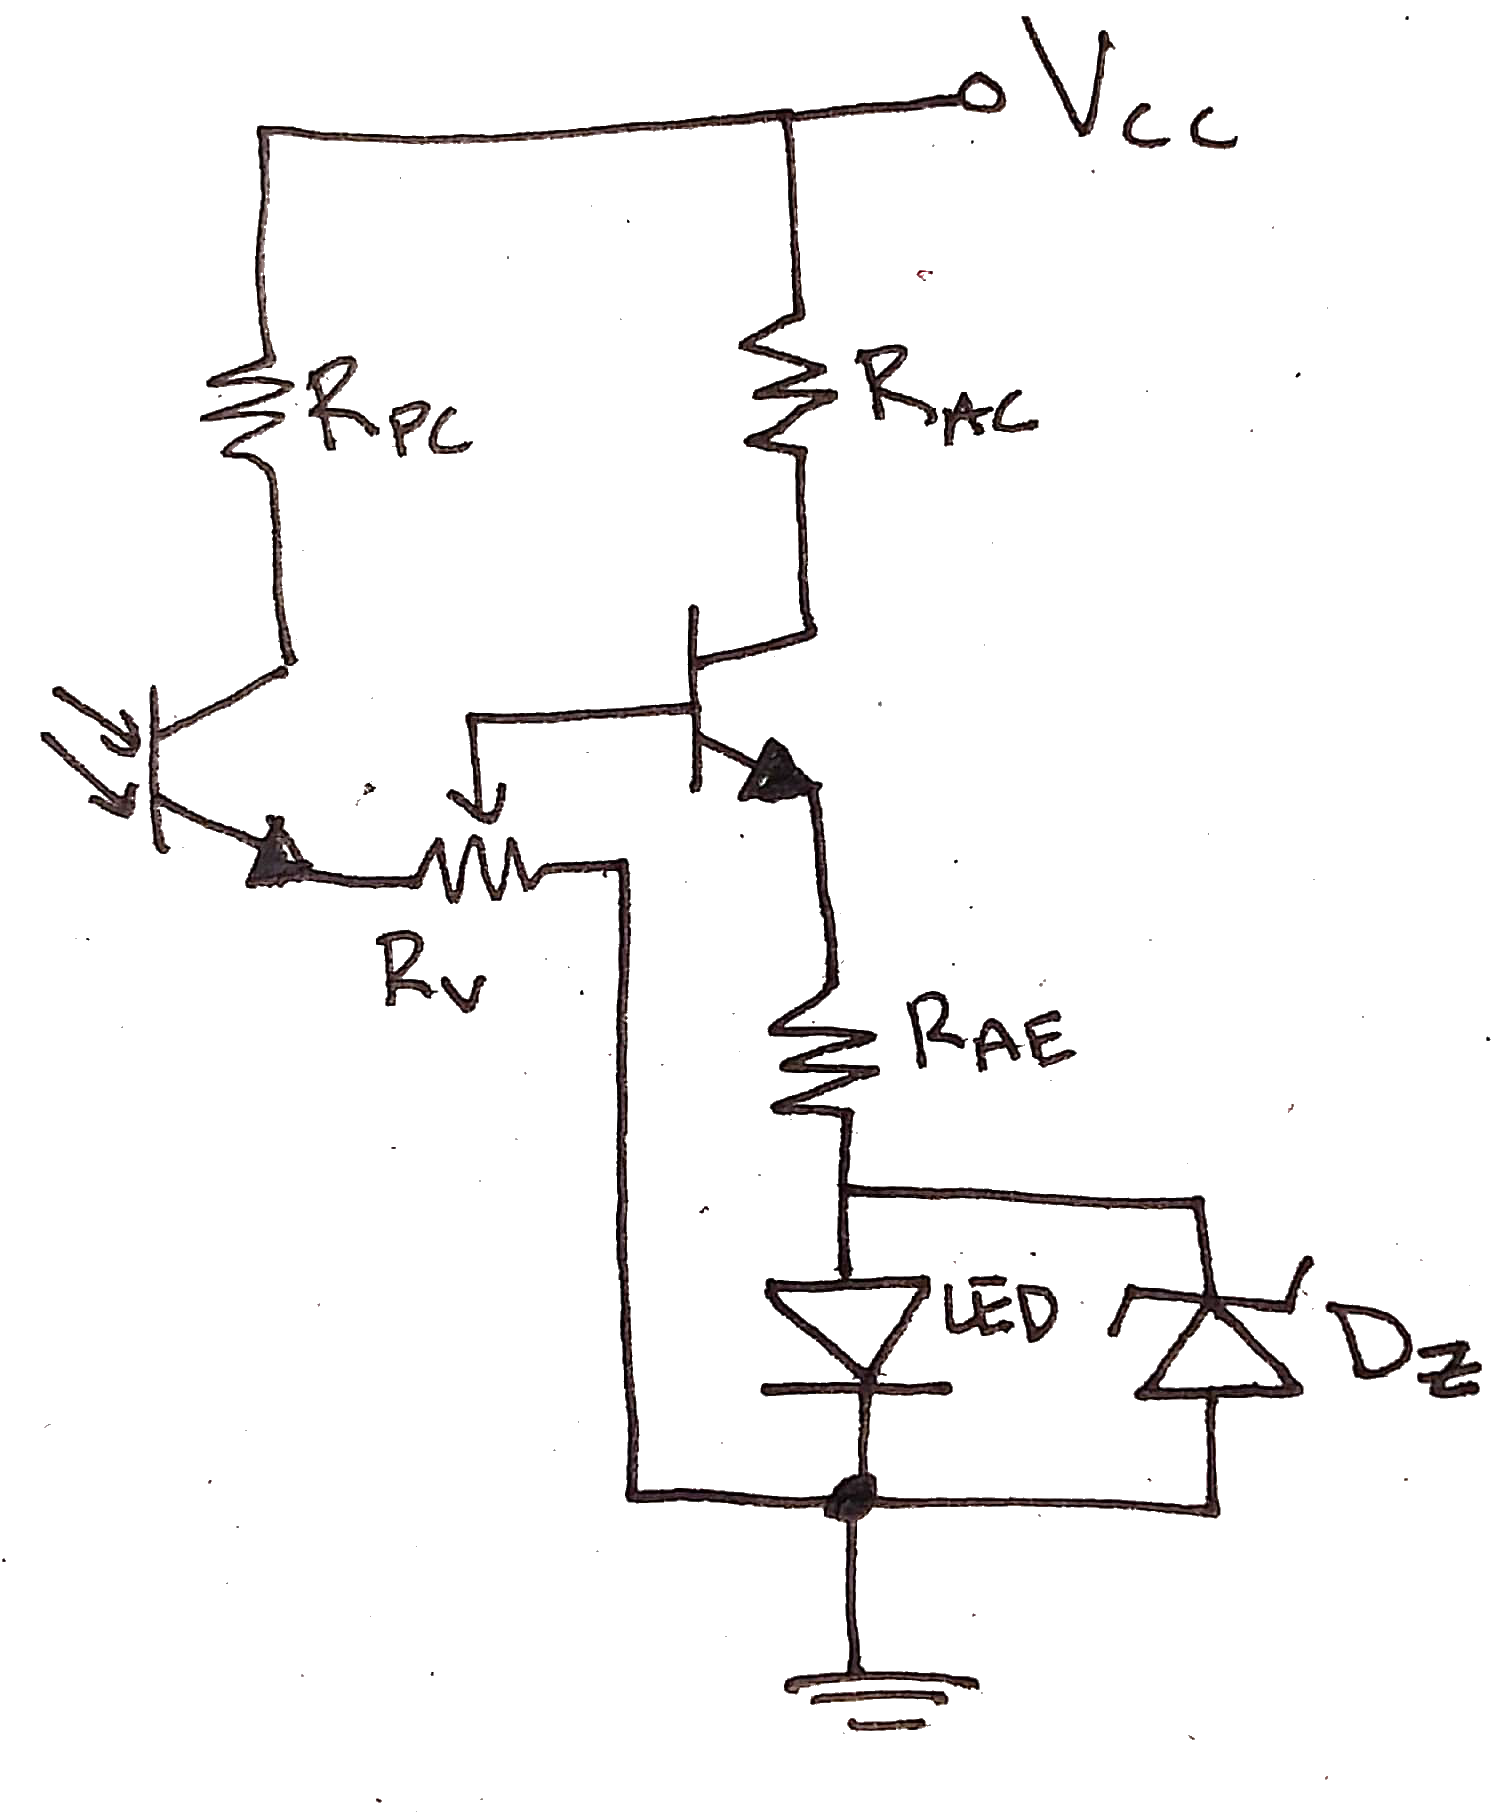
\includegraphics[width=2.5in]{c11.png}
	\caption{Infrared Detector Circuit With LED Output (Lab 11)}
	\label{fig1}
\end{figure}


You can see this circuit in action here: \url{https://mediaspace.minnstate.edu/media/Photodetector/1_ssmrx1ba}

I thought adding a zener diode, reverse biased, in parallel with the LED would define the range of our output, it didn't seem to do so fully. It's not necessarily clear in the video, but the brightness of the LED would change based on the distance of the remote, although less so than without the zener diode in place. This remote also only has a range of roughly 3.5 feet, which in practice is unlikely the case. I suspect this a result of the LED and Zener Diode fighting each other on voltage drops, but being parallel need to agree. If the led had an additional resistor in place, to take the additional voltage drop required by the zener diode, I suspect this circuit would be much closer to our expected result.


%\begin{thebibliography}{99}
% The numeral (here 99) in curly braces is nominally the number of entries in
% the bibliography. It's supposed to affect the amount of space around the
% numerical labels, so only the number of digits should matter--and even that
% seems to make no discernible difference.
%Not Requested
%\end{thebibliography}

\end{document}
